\chapter{测试驱动开发} % Introduction chapter suppressed from the table of contents

\hypertarget{ux6d4bux8bd5ux9a71ux52a8ux5f00ux53d1}{%
\section{测试驱动开发}\label{ux6d4bux8bd5ux9a71ux52a8ux5f00ux53d1}}

开发人员问:为什么要这么做?写完程序后,然后再写测试用例,不是更正常吗?

\hypertarget{ux4e3aux4ec0ux4e48ux6211ux4eecux8981ux6d4bux8bd5ux9a71ux52a8ux5f00ux53d1}{%
\subsection{为什么我们要测试驱动开发}\label{ux4e3aux4ec0ux4e48ux6211ux4eecux8981ux6d4bux8bd5ux9a71ux52a8ux5f00ux53d1}}

\textbf{精益}是敏捷中很核心的概念。最近发生的一件事帮我回答了以上问题,也让我体会到TDD与精益的概念是如何协同的。

我有一位拥有三十多年电机工程经验的老同学李先生,他在对Linux的研究方面一直都很有兴趣,这几年又开始玩树莓派,目前他对此非常精通。

最近我找到他,希望在树莓派上安装 Ipython, Jupyter Notebook
等开源应用软件。一直以来,李先生的理念就是尽量用最简单、最轻易的方法去解决客户的问题,而不是浪费资源。

例如,95年开始尝试建立 wiki
服务器给客户使用的时候,他就建议我用树莓派来建:\\
他说:''树莓派不仅省电而且快,也不知道你这个概念是否持久,我不会浪费时间------在大型服务器上安装
Linux +Mediawiki ,如果你觉得这(树莓派)可以,
便继续用。如果觉得它性能不够了,下一步我帮你换更大型的服务器。''

%\href{文件:树莓派2.jpg}{300px}

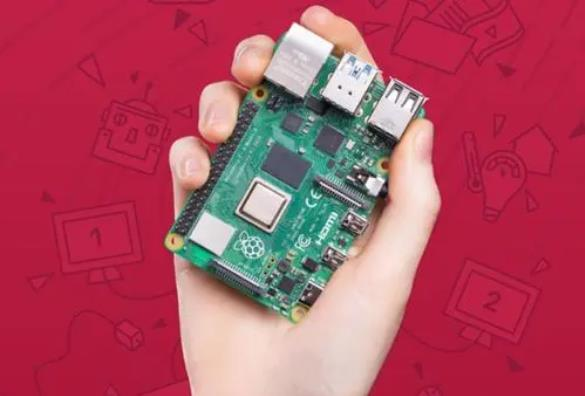
\includegraphics[width=6cm]{树莓派2.jpg}

---直到现在, 已经7
年了,我们一直还是继续用树莓派来协助评估(树莓派从原来的Pi2(1G内存),现在已经是P4(4G内存),已经服务超过百家客户了,这证明他的思路是对的。

回到我刚才说要安装 Jupyter Notebook
,他安装好那个程序包后,一直没动。我问他什么原因?他说:``
很简单,我不熟悉软件工程,也不懂如何测试。
肯定要找你测试一下,我才知道有没有做错。这样可以避免无谓的返工。''

所以我们就约好周日我回到到办公室跟他远程测试。

李先生打开树莓派后,我用VNC客户端进入他的树莓派,打一些最基本的 Ipython
指令,验证没问题。

下一步我要跑一些比较复杂的、要用到 Pandas 包的 Python
程序,却发现还没有安装Pandas包。他马上到网上去找安装介质以及树莓派如何安装
PANDAS 的方法。
处理好后,我再跑对应的程序,都跑通了,包括之前跑过的指令。前后两个小时,按本来计划,测试成功。

我回想一下,其实他的思路就是精益。用有限资源、以最低投入,达到客户要求,不多做。每当李先生做完一步,如果没有通过测试,就不会浪费时间走下一步------这也是精益和测试驱动开发的原理。

\hypertarget{ux6bcfux5c0fux6b65ux9a8cux8bc1}{%
\subsection{每小步验证}\label{ux6bcfux5c0fux6b65ux9a8cux8bc1}}

工程类的本科生都要在最后一年做毕业项目。当时,1983年,导师建议我们尝试参考一些常用的语言发声算法,在专门做信号处理的芯片上写程序,读出一些英文字或句子(与现在不同,当时这项技术还没有成熟,很多大学还在研究),虽然我预计有不小的技术难度,但觉得这很先进,很感兴趣,便与另一位同学合作,开始制定项目计划。

我们很努力,全情投入,一面要研究语言发声的算法,一面还要并行设计电子线路和软件等。我们用了
2 \textasciitilde{} 3
个月的时间做了整个电子线路板的硬件,同时还设计了整个软件架构,并使用计算机模拟,验证每个字实现算法后的发声效果,因为最后一年课程很多,时间过得很快,从9月开始准备一直到次年3月,软硬件的设计与开发终于都完成了,但是不知道什么原因就是没有声音,更不要说能读出一些字和句子了,最后项目以失败告终。

在这之前的一年,我有幸在大学的第三年进入大东电报局(Cable \&
Wireless)实习(当时香港的所有国际通讯都是经过大东),实习的部门(负责电报业务运维)正如火如荼开发一套新的电脑系统以取代本来基于UNIVAC的电报系统,总工程师让我用半年时间,在一个微机上编程,做一个系统,以从那些电脑上收集重要信息,如果发现异常就警报。头三个月都是花精力做整个系统设计,也买了一些展示电子版,准备用来展示,但由于经验不足,半年后最终什么都展示不出来。

到了2000年,在我兼读软件工程硕士课程时,开始接触到敏捷开发,才了解到两次项目失败的主因:不应该花大量时间去做前期设计------希望有一个完美的设计,而是应该一步一步迭代,先做一些最基本的简单功能,逐步优化。例如,在我的毕业项目中,应该先做出最基本的硬件、软件,起码能够发出声音,因为没有前人做过,整个项目是从未做过的实验。

敏捷大师Dave Thomas 先生在2015 演讲里提出敏捷软件开发的核心是:

\framebox{%
\begin{minipage}[t]{0.97\columnwidth}\raggedright
\begin{enumerate}
\tightlist
\item
  向你的目标迈出一小步。
\item
  从反馈调整你的理解。
\item
  重复。
\end{enumerate}

\begin{itemize}
\tightlist
\item
  当两种或以上选择的价值大致相同时,选一条让未来更容易修改(软件)的路径。
\end{itemize}\strut
\end{minipage}}


这些经历让我体会到为什么我们在写程序时,必须先想一下该怎么测试。

\hypertarget{ux7528tddux5f00ux53d1ux7a0bux5e8f}{%
\subsection{用TDD开发程序}\label{ux7528tddux5f00ux53d1ux7a0bux5e8f}}

程序员问:为什么我们要针对这么小的部分都做单元测试?

答:

\begin{enumerate}
\tightlist
\item
  小的单元测试容易写,比较简单,不会花费很多时间。
\item
  因为任何程序都会按时间变化,越来越复杂。有了单元测试,后面的测试就有依据,知道改动是否出错。没有单元测试的话,就没有信心去改程序,不知道是否没问题。
\end{enumerate}

\begin{description}
\item[]
\begin{description}
\tightlist
\item[]
(这和我们工程的概念一样,把工程细分,每个子系统都要确保质量达标,尽量找出缺陷,才进行下一步。)
\end{description}

如不相信请看看我从头学编程的实例:
\end{description}

\framebox{%
\begin{minipage}[t]{0.97\columnwidth}\raggedright
Shiny是专门用于制作互动看板。我看它的Gallery里有很多现成看板,也提供R代码,我就找了某些例子,都能跑通。但若想增加功能,因不熟识Shiny的
R 编程便跑不通了。下决心按官网推荐的参考书开始学习。

星期六下午开始学习如何用R语言写Shiny程序,参考一本Shiny课本学习第一章就有一个实例,Shiny
的 App.R 代码架构分UI部分,和服务器(Server)部分。

先跑两个最基本测试,验证shiny服务器平台可以在本地展示(因为有时候,配置不匹配,展示不出来,需要先重启):

\begin{description}
\tightlist
\item[]
\textgreater{} library(shiny) \# 安装Shiny包

\textgreater{} runExample("01\_hello") \# Shiny包自带的示范例子

\textgreater{} runApp("tst\_shiny") \# 我之前按另一本R参考书打的app.R
示例
\end{description}

16:37 练习1:本来要写最简单 "Hello
world",只需要在框架里加一句,我觉得太简单了,就直接跳到下一个练习,这个程序是打开页面用户输入选择其中一个现有的数据包,然后打开显示,也很简单,我基于框架(UI
+ Server)
加了9行代码,报错,想不到错在哪里。报语句不通,想来想去,没办法,我就把那些内容都删掉,从最基本的"Hello
world"开始,但还是报错,我仔细看代码,原来我打错了基本框架里一个字,改正后"Hello
world"可以跑通。我就继续写练习二"Hello
world",展示数据包数据,又报错。仔细看代码,原来我又打错一个字 (label
写错了),改正后能跑通。

17:16 进一步做第一章后面的其他练习,Shiny有一个很好的功能,叫 reactive
expression: 类似 function
功能,防止程序员重复代码,(如果重复代码,难以维护,常常会出错,重复代码都应该改成
reactive expression
来调用,避免拷贝粘贴代码。)所以我先按练习需求,先把本来的程序(有重复代码)跑通。我然后按练习要求,加入
reactive , 取代重复语句。最后加了reactive
的程序也跑通,我看看时间是17:40,刚好一个小时。

总共只是写了大概三十行代码,但我每写一小部分都会测试,总共做了五轮编写测试循环。每位程序员都应该是按同样思路:软件开发项目都应该分成小步,每一步正式通过才走下一步,才避免走弯路。只是写完代码,没通过测试,不算完成;如果你写完一个模块没有通过单元测试,你是无法证明你写的代码是正确,不算负责任的程序员(单元测试与产品集成会在后面详细介绍)。
\strut
\end{minipage}}

网上有关于是否要TDD的争论:

\begin{itemize}
\tightlist
\item
  一派是坚持要先写测试用例,再写编码。
\item
  另一派觉得TDD太多余,如果功能测试做得全,也不一定要有单元测试。
\end{itemize}

这个争论让我想起以前教ACP敏捷管理的一个原则,叫``守 破 离''。

\hypertarget{ux5b88-ux7834-ux79bb}{%
\subsubsection{守 破 离}\label{ux5b88-ux7834-ux79bb}}

英文翻译成 ``Shu -- Ha -- Ri '' ,意思是学习合气道,要先从基本功出发
(守),按规则一步一步做。当你理解以后,就能融会贯通
(破),融合管理到一定境界就是大师级了 (离)。

像宫本武藏(江户时代著名剑术家)一样,一生赢了六十多场决斗,然而到了晚年,他在《五轮书》中总结,不要局限于某种刀法,最重要是抓住原理。

敏捷大师 Mr Cockburn 有一次到企业做 Class-responsibility-collaboration
(CRC) card 咨询培训,因为他很熟悉 CRC
方法,他觉得只要有助于面向对象设计,不一定要按原本的方式,可以简化。但学生都不熟悉,一直在问``请你告诉我们从头到尾,每一步如何做,我们照着做''大师没办法,最终按最原始的方法,一步步来教如何去做,学生才能懂,这是守破离的``守''。

TDD测试驱动开发也一样,把TDD看成``守'',当没有概念的时候,还是要从最基本的概念入手,我们每个程序都应该有测试,所以自然的顺序是先写测试用例,再写代码,这也能更好地帮助你理解程序的功能。

所以TDD就是做好程序基本功的基础,当你已经掌握这些基础了,就可以灵活处理,可能不一定要每次先写测试用例,但底线是每个代码都要有单元测试。

但是有些人觉得,只要有功能测试,单元测试可以不做。

功能测试是黑盒测试,从客户的角度测试总体功能,无法真正判断代码是否正确。反过来,单元测试是白盒测试,从代码的功能角度,验证代码是否正确,所以功能测试是不能替代单元测试的。尤其是当代码有功能上的变化时,就更需要有单元测试来验证这些改动是否有误,所以单元测试的复用率非常高。

大家正在越来越多地使用自动集成工具,如果有单元测试,那么每天的自动集成就不仅仅是看编译是否通过,还需要通过单元测试,才能更好地保证代码质量,这就是很有效率的回归测试。(回归测试:为避免因代码修改,导致原先通过的测试不通过,所以之前通过的测试用例也要重复再测。如果手工测试,为了节省测试时间,只重跑部分重要测试,但如果自动化,就可以轻松地重跑所有测试用例。)

\hypertarget{ux5355ux5143ux6d4bux8bd5ux4e0etddux7684ux597dux5904}{%
\subsection{单元测试与TDD的好处}\label{ux5355ux5143ux6d4bux8bd5ux4e0etddux7684ux597dux5904}}

上周在杭州跟一位资深的开发主管对话,他回国前在日本工作了接近10年,他说很佩服日本注重开发质量,例如很注重单元测试,所以回国后在团队严格要求要有单元测试。

我问:现在有很多静态代码检测,为何还要单元测试。

他答:目的不同,静态代码检测只是用过去的历史经验去检查常见的语法、命名问题,但如果是设计本身的逻辑问题就无法查出。
以他多年的经验,必须通过单元测试才有信心确认这个程序是否正常,单靠集成测试、功能测试是无法确保程序的每一部分都是正常的。所以他严格要求团队,代码经过检验后(自动静态检验或代码走查),还必须做单元测试才能进入下一步的集成、系统测试。

单是靠集成测试、功能测试是无法确保程序每一部分都正常。

他还说TDD 有三点好处:

\begin{enumerate}
\tightlist
\item
  让开发人员在编码前去理解设计和需求。
\item
  让开发人员知道代码可验证性的重要。
\item
  强迫开发人员主动与设计和需求人员沟通,否则无法设计出单元测试用例,但TDD
  对团队成员素质要求较高。
\end{enumerate}

\hypertarget{ux7ed3ux675fux8bed}{%
\subsection{结束语}\label{ux7ed3ux675fux8bed}}

开发人员用TDD编程,体现每走一步前必须验证通过,减少返工,精益思路,是中初级程序员健康成长之路,养成好习惯。

但若你是九段高手,因已经过了以上基本训练阶段,可能便不再需要,好比合气道``守
破 离''成长路径。

有些敏捷大师,已经累积有20年以上编程经验,例如上面提到的Thomas先生,他已经很少写单元测试,因为他觉得已经不需要依赖单元测试来验证代码是否正确。

\begin{description}
\item[]
\begin{description}
\tightlist
\item[]
-\/-\/-===\textless{}\textless{}\textless{} END
\textgreater{}\textgreater{}\textgreater{}===-\/-\/-
\end{description}
\end{description}


